\documentclass[11pt, oneside, titlepage, a4paper]{article}
\usepackage[utf8x]{inputenc}
\usepackage[T1]{fontenc}
\usepackage[francais]{babel}

\usepackage{graphicx}
\usepackage{hyperref}
\usepackage[sectionmark, fancysections]{polytechnique}
\usepackage{url}

\title{Rapport de stage en entreprise}
\subtitle{Bloomberg L.P. -- Recherche et Développement}
\logo{logo.jpg}
\author{\textsc{Cornet Alexandre}}
\date{\today}

\begin{document}
\maketitle
\section*{Résumé opérationnel}
\begin{small}
Bloomberg L.P. est une compagnie technologique et financière qui offre ses services aux acteurs des marchés financiers. Elle doit sa renommée au Bloomberg Terminal, son produit-phare et leader de son secteur. Le Terminal est un système informatique donnant accès au Bloomberg Professional Service. Ce service permet aux professionnels des marchés financiers et de l'industrie d'accéder en temps réel aux données essentielles dans leur activité. Le coeur de l'activité de Bloomberg L.P. consiste donc à collecter, normaliser et distribuer toutes les données indispensables aux professionnels du secteur.

L'entreprise est également une référence dans le milieu de l'information économique et financière. Bloomberg News est en effet devenue en quelques années une des plus grandes agences de presse au monde, et diffuse ses informations via de nombreuses plateformes: internet, télévision, radio, presse écrite.
\\

Dans ce contexte, le département Recherche et Développement (R\&D) a pour mission de concevoir, développer et déployer les technologies nécessaires pour distribuer les informations disponibles dans le système. Les utilisateurs du Terminal évoluent dans un contexte extrêmement compétitif où le temps est crucial. Ces technologies doivent donc garantir une disponibilité permanente et instantanée aux données, ainsi qu'une expérience d'utilisation la plus proche possible des besoins des clients.

Le Bloomberg Professional Service dispose entre autres d'un système de messagerie instantanée, Instant Bloomberg (IB). Cette fonctionnalité est extrêmement populaire et largement utilisée par les usagers du Terminal. Ces applications sont nombreuses: coordination entre collègues, propositions d'achat ou de vente sur les marchés ou encore diffusion d'informations critiques dans des chats réunissant plusieurs centaines d'utilisateurs. Depuis sa création, IB s'est donc imposé comme un outil indispensable pour les professionnels des marchés financiers.
\\

Lors de ces deux mois passés à Bloomberg, j'ai travaillé au sein d'une des quatre équipes de R\&D responsables d'IB: l'équipe IB2 Distribution. Cette équipe a pour rôle de garantir la distribution des messages depuis le réseau global jusqu'aux utilisateurs. Au bout de la chaine de distribution, un composant reçoit l'ensemble des messages diffusés dans le réseau. Il a ensuite pour rôle de publier chaque message dans un emplacement de mémoire dédié à son destinataire, appelé table. Cette table est enfin lue par l'ordinateur, la tablette ou le téléphone de l'utilisateur pour afficher les messages à l'écran. Ce composant, ou application, sera nommé IB Publisher dans la suite de ce rapport.

Dans le but d'améliorer sa fiabilité et de supporter de nouvelles fonctionnalités, IB Publisher est actuellement fortement restructuré. Si l'équipe dispose de tests garantissant le bon fonctionnement des sous composants de l'application, aucun test ne permet de prouver qu'ils satisferont le cahier des charges global une fois assemblés. Ces tests, appelés tests d'intégration, sont pourtant cruciaux pour adopter un procédé itératif de développement et pour garantir la fiabilité du produit à toute étape de la production.
\\

Dans ce contexte, ma mission consistait à développer un environnement permettant de réaliser des tests d'intégration sur IB Publisher. Il s'agissait donc de créer un nouvel outil capable de simuler l'envoi de messages dans le réseau et de vérifier que les résultats obtenus sont conformes aux exigences.

Au terme de neuf semaines de travail, j'ai pu délivrer à l'équipe une première version fonctionnelle d'un tel outil. Dans les mois à venir, cet outil sera complexifié et intégré dans l'environnement de production d'IB. Ainsi, les dernières modifications apportées à IB Publisher pourront être testées chaque nuit avant d'être mises en production.
\end{small}
\newpage
\tableofcontents
\newpage
\section{Introduction}
Attiré depuis plusieurs années par l'ingénierie logicielle, je souhaitais effectuer un stage de développement informatique. Toutefois, je n'avais pas d'idée précise quant au secteur d'activité (industrie, finance) dans lequel je souhaitais évoluer.

J'avais également pour projet de perfectionner mon anglais et je devais m'absenter quelques jours pour participer au défilé du 14 Juillet. Pour ces raisons, Londres me paraissait comme étant une destination intéressante.
\\

Je suis tout d'abord rentré en contact avec l'entreprise Amadeus, qui offre ses services aux professionnels du secteur du transport aérien. Cependant, la compagnie proposait des opportunités de stage uniquement à Antibes, ce qui m'a conduit à mettre cette offre en attente.
\\

J'ai découvert Bloomberg L.P. au fil de mes recherches. À l'intersection de l'informatique et de la finance, le programme de stage proposé par la compagnie m'a tout de suite attiré. J'ai en effet toujours été intéressé par l'économie et la finance  sans pour autant les avoir étudiés. Cette opportunité m'a donc semblé être un bon compromis entre la découverte du développement industriel de logiciels et la découverte du secteur financier.

Je suis alors rentré en contact avec Laurent Romieux, X1999, actuellement chef d'une équipe de Recherche et Développement dans les bureaux londoniens de Bloomberg L.P.. Membre de l'équipe de recrutement des stagiaires et en voyage de recrutement à Paris, il m'a proposé de passer un entretien dans les bureaux parisiens de la compagnie.
\\

Afin de multiplier mes opportunités, j'ai également postulé et passé un entretien pour un stage en R\&D à la Banque de France. Bien que très bien défini, le cadre de ce stage ne me paraissait pas suffisamment dynamique. De plus cette opportunité ne me permettait ni de perfectionner mon anglais ni d'évoluer dans un environnement multiculturel.

Ma préférence s'est donc portée vers Bloomberg et j'ai eu la chance de rejoindre une grande compagnie, mondialement reconnue comme leader de son secteur. 
\\

Le but de ce rapport est avant tout de décrire l'environnement dans lequel j'ai évolué cet été ainsi que le projet sur lequel j'ai travaillé. 

Les enseignements que cette expérience m'a apporté seront développés plus en détails lors de la soutenance orale. J'aurai alors plus de recul sur mes réalisations, mes erreurs et mes réussites.
\newpage
\section{Bloomberg L.P.}
	\subsection{Présentation historique}
Bloomberg L.P. est une compagnie technologique et financière spécialisée dans les services aux acteurs des marchés financiers et de l'industrie. Elle fut fondée en 1981 par Michael Bloomberg, maire de New York de 2002 à 2013, avec l'aide de Duncan MacMillan, Charles Zegar et Thomas Secunda. L'histoire de la compagnie est fondamentale pour en comprendre le succès mais surtout l'identité et les valeurs qui sont décrites plus loin.
		\subsubsection{De Innovative Market System à Bloomberg L.P.}
À l'âge de trente ans, Michael Bloomberg devient un des associés de la banque d'investissement américaine Salamon Brothers. Il y dirige le service de trading d'actions (equity trading) puis le service de développement des systèmes informatiques, où il conçoit des outils d'aide aux professionnels des marchés financiers. Il réalise alors que Wall Street constitue un vaste marché pour des systèmes délivrant des données financières de haute qualité, disponibles instantanément et sous une forme exploitable.

En 1981, le fonds d'investissements Phibro Corporation fait l'acquisition de Salamon Brothers. Bloomberg est alors écarté mais reçoit dix millions de dollars en échange de ses parts dans l'entreprise. Il les utilise pour fonder sa compagnie, Innovative Market System (IMS), avec la participation de trois autres ex-employés de Salamon Brothers. Leur projet est d'utiliser les dernières technologies pour développer un outil capable de délivrer des données financières en temps réel ainsi que d'autres outils d'analyse. Secunda, mathématicien, est responsable de rassembler et de saisir les données distribuées dans le système. Zegar est chargé d'écrire le logiciel. MacMilan et Bloomberg sont quant à eux chargés des ventes, Bloomberg assurant également la fonction de président.
\\

L'idée brillante de l'équipe est de répondre aux besoins et aux questions des professionnels des marchés par des fonctions. Au lieu de classifier les informations disponibles dans le système sous forme d'une arborescence, ils basent leur outil sur le même principe de fonctionnement que celui d'un terminal d'ordinateur: à chaque demande correspond une ligne de code, une fonction, suivie de l'objet sur lequel appliquer cette demande, les paramètres. Ainsi, pour afficher le taux de change entre le dollar et la livre, il suffit d'entrer : \og USDGBP Currency \fg{}.

La version actuelle du Terminal est encore basée sur ce principe, qui fait la simplicité d'utilisation et l'efficacité à l'origine du succès du Terminal.
\\

Environ un an plus tard, Michael Bloomberg effectue la première vente de la compagnie et installe vingt-deux terminaux pour la banque d'investissement américaine Merrill Lynch. La banque investit alors trente millions de dollars dans la compagnie, acquérant ainsi trente pour-cents du capital, et met à disposition son réseau de clients.

Le contexte de cette vente, acte fondateur de l'entreprise, constitue une excellente manifestation de l'identité de Bloomberg L.P.. Dans les heures précédant la présentation de Bloomberg dans les bureaux de Merrill Lynch, un bug s'est en effet glissé dans le code du Terminal, rendant le système fortement instable. Conscient qu'il ne pourrait obtenir un nouvel entretien, Bloomberg décide de tenter sa chance et de prendre le risque d'un crash pendant la démonstration. Pendant les heures précédant la présentation, l'équipe s'affaire à trouver un enchainement de taches ne provoquant aucun bug, que Bloomberg reproduisit avec succès lors de sa présentation. Plus de quarante ans après cette vente, ce gout du risque propre à une jeune start-up demeure toujours une des valeurs fortes de la compagnie.
\\

En 1986, IMS est renommée Bloomberg L.P. et 5000 terminaux ont été vendus, constituant plusieurs années avant l'apparition d'Internet un vaste réseau de machines inter-connectées. La compagnie fut donc depuis sa création, et demeure encore, un grand acteur dans le monde de l'innovation technologique.

\begin{figure}
\begin{center}
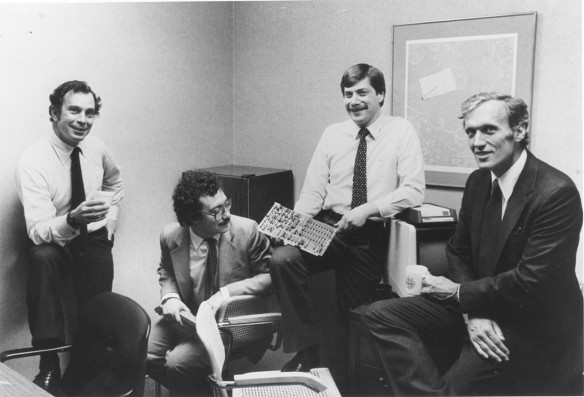
\includegraphics[scale=0.37]{creation.jpg}
\caption{Les fondateurs de Bloomberg L.P.}
\end{center}
\end{figure}
		\subsubsection{La diversification des services}
Dans les années qui suivent, la compagnie lance sa plateforme de trading, son service de messagerie électronique et son service de presse.
\\

Bloomberg News est créé en 1990 par Michael Bloomberg et Matthew Winkler, alors journaliste au Wall Street Journal, et qui assure depuis le poste d'éditeur en chef. L'objectif est de diversifier les informations disponibles sur le Terminal mais aussi de faire connaitre Bloomberg en publiant publiquement une partie de ces articles. L'agence propose une nouvelle forme d'information adaptée aux acteurs des marchés financiers, concise et efficace. La première équipe est formée de six personnes.

Bloomberg News connaît alors une croissance rapide et conquiert toujours plus de supports: internet avec la création de Bloomberg.com en 1993, la télévision, la radio et enfin le monde conventionnel de la presse écrite. En particulier, l'agence est mondialement renommée comme l'une des plus fiables et une des plus rapides. Ainsi la phrase \og If that's on Bloomberg, that's true.\fg{} est presque devenue un adage sur les marchés, et l'agence devance parfois ses concurrents de plusieurs heures dans la publication d'informations, comme le décès de Margaret Thatcher en 2013.

L'agence emploie aujourd'hui plus de 2300 journalistes répartis dans plus de 150 bureaux et 73 pays, publiant plus de 5000 articles chaque jour.
\\

Bloomberg Tradebook fut créé en 1996 afin d'offrir aux utilisateurs du Bloomberg Terminal la possibilité d'effectuer des transactions sur les marchés financiers directement depuis le Terminal. Derrière la plateforme utilisée par les usagers opère donc une agence de courtiers (broker).

Permettant d'abord d'accéder uniquement aux marchés américains, la plateforme permet d'effectuer des transactions sur les marchés asiatiques depuis 1999 et sur les marchés européens depuis 2000. Tradebook offre aujourd'hui l'accès à plus de 110 marchés répartis dans 44 pays.

La plateforme est particulièrement populaire auprès des entités financières de taille moyenne, trop petites pour pouvoir payer les frais d'accès aux marchés.
\\

Ces produits demeurent phares pour la compagnie, en particulier le Terminal qui est parfois comparé au soleil dans le système solaire de Bloomberg. Un des plus grands atouts du Terminal est la diversité des services qui lui sont intégrés, offrant aux professionnels tous les outils nécessaires à leur activité dans une interface unique.
		\subsubsection{Situation actuelle}
Bloomberg L.P. a connu une croissance fulgurante depuis la fin des années 80. De 10,000 terminaux en 1990, les ventes passent à plus de 150,000 terminaux en 2000. Ce chiffre sera doublé au début des années 2010 malgré une stagnation des ventes suite à la crise des subprimes. La compagnie a aujourd'hui retrouvé une croissance supérieure à celle d'avant-crise et on compte plus de 325,000 terminaux dans le monde.
\\

Bloomberg L.P. demeure depuis sa création une société privée, ce qui explique notamment le peu de données disponibles sur son activité.

Suite à l'investissement initial de Merrill Lynch, la compagnie est détenue à 58\% par Michael Bloomberg, 30\% par la banque d'investissement américaine et 12\% par les trois autres cofondateurs (4\% chacun). Les seules évaluations de la valeur de la compagnie sont le fait du rachat des parts de Merrill Lynch par Michael Bloomberg. En 1996, il fait l'acquisition d'un tiers de ces parts pour une valeur de 200 millions de dollars, évaluant ainsi la compagnie à deux milliards de dollars. En 2008, en pleine crise des subprimes, Merrill Lynch accepte de céder l'ensemble de ses parts pour 4,43 millions de dollars, évaluant la compagnie à 22,3 milliards de dollars.

Michael Bloomberg, qui avait quitté ses fonctions de président directeur général pour se consacrer pleinement à la mairie de New York, a repris son poste au début de l'année 2014.
\\

Le prix du Bloomberg Terminal varie de 20,000\$ pour tout contrat supérieur à deux abonnements à 24,000\$ pour un abonnement unique. Le Terminal étant de loin la principale source de revenus de la compagnie, on estime le chiffre d'affaire annuel de Bloomberg L.P. à 7,5 milliards de dollars l'année dernière.

Bloomberg L.P. demeure leader dans le secteur de la distribution de données et d'informations aux marchés financiers. La compagnie se partage avec son principal concurrent,Thomson Reuters, plus de 90\% du marché. Aucun autre concurrent ne représente plus de 3,6\% du marché.

Historiquement, le Bloomberg Terminal était essentiellement utilisé dans le milieu du fixed income (revenus fixes) par des professionnels échangeant des bonds (dettes). En parallèle, l'outil Eikon proposé par Reuters était traditionnellement utilisé pour obtenir des informations sur le marché des actions. Cette tendance s'est progressivement affaiblie et le Terminal s'est imposé comme outils de référence dans tous les milieux du secteur.

On estime la part de marché de Bloomberg à 54\% contre 37\% pour Reuteurs, avec 190,000 abonnés en 2013. À titre indicatif, le logiciel de Reuters coute 21,600\$ par an, prix comparable à celui du Terminal.
\\

\begin{figure}[h]
\begin{center}
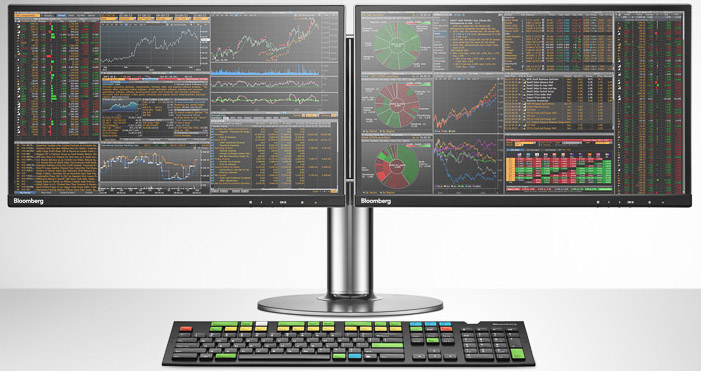
\includegraphics[scale=0.3]{terminal.jpg}
\caption{Le Bloomberg Terminal commercialisé de nos jours}
\end{center}
\end{figure}
Bloomberg L.P. regroupe aujourd'hui plus de 15,000 employés répartis dans 192 bureaux à travers le monde et la compagnie embauche massivement dans tous les départements. Ainsi, la moitié de mon équipe a été recruté il y a moins d'un an et sur les 150 stagiaires présents à Londres cet été, plus de la moitié recevra une offre d'emploi.

Le siège de la compagnie est situé à Lexington Avenue à New York où sont basés plus de 6,000 employés. Les bureaux Londoniens réunissent quant à eux 4,000 employés sur trois sites: deux sites voisins au nord de la City et le troisième dans le quartier d'affaires de Canary Wharf.
	\subsection{Identité et Culture}
Bloomberg L.P. possède une culture et une identité très fortes et très influencées par le fondateur de la compagnie, Michael Bloomberg. Cette identité repose sur deux piliers: créer un environnement de travail le plus enrichissant possible pour les employés, et rendre de façon juste et durable les profits réalisés par la compagnie.

Toutes ses valeurs sont présentées dès le premier jour à chaque employé. Toutefois, quelques semaines m'ont été nécessaires pour réaliser à quel point elles sont profondément ancrées et fondamentales dans le quotidien des employés.
		\subsubsection{Bloomberg Values} \label{values}
La culture de Bloomberg se matérialise autour de huit valeurs qui démontrent la recherche de transparence, de collaboration et de créativité dans le quotidien des employés. Ces valeurs prennent leur sens au niveau d'un employé, d'une équipe ou de la compagnie tout entière. Elles sont les suivantes: connaître le consommateur, travailler dur, agir vite et avec jugement, être audacieux, apprendre de ses erreurs, collaborer, suivre l'exemple et agir avec intégrité.

Comme pour chaque employé, ces valeurs m'ont été présentées le jour de mon arrivée à Bloomberg. Pour être tout à fait honnête, je suis arrivé à Londres avec quelques a priori sur le monde des grandes compagnies financières. J'ai donc d'abord cru qu'il s'agissait d'un discours de la première heure, auquel seules les ressources humaines croient vraiment. Au fil de mes expériences dans la compagnie cependant, j'ai pu réaliser qu'il s'agissait d'une réalité perceptible au quotidien et que ces valeurs étaient les piliers d'un état d'esprit partagé par tous les employés.

Les exemples de leur manifestation sont nombreux, aussi n'en décrirais-je que quelques-uns.
\\

Celle que j'ai le plus observée et qui a été clé dans la réussite de ma mission est sans aucun doute le souci de la collaboration. Au sein de mon équipe, tout le monde était prêt à mettre son propre travail de côté, quelques minutes ou plusieurs heures, pour m'aider à résoudre un problème technique, m'expliquer un nouveau concept ou réfléchir aux prochaines étapes de mon travail. De mon premier jour jusqu'à mon départ, j'ai toujours su que j'avais le soutien de toute l'équipe et que je pouvais leur communiquer toutes mes interrogations.
\\

Une des valeurs les plus fortes et des plus fondatrices de l'identité de Bloomberg est sans doute l'audace (et donc parfois apprendre de ses erreurs par la suite!). Comme évoqué ci-dessus, la première vente de la compagnie n'aurait pas eu lieu sans le cran de ses fondateurs. La compagnie a depuis conservé cet esprit proche de celui des jeunes start-up, s'efforçant de toujours trouver de nouvelles idées et d'innover.
\\

Un autre exemple marquant de cet état esprit m'a été décrit lors d'une présentation proposée à l'ensemble des stagiaires. Chaque vendredi midi, quelques employés venaient nous présenter leur département, leur quotidien et aussi nous raconter leur histoire à Bloomberg. L'actuel directeur du département Global Data EMEA (décrit plus bas), a d'abord commencé à travailler dans le service d'aide à la clientèle.

Ce service est essentiel pour les utilisateurs, car il est parfois difficile de trouver comment accéder à une donnée. À l'origine, il était joignable uniquement par téléphone. Le jour de son entretien d'embauche douze ans plus tôt, Bloomberg lançait une fonctionnalité désormais connue de tous les utilisateurs du Terminal: deux appuis sur la touche HELP du clavier ouvrent une fenêtre de discussion instantanée avec un technicien.

À son arrivée à l'étage du service client, cette fonctionnalité était sur le point d'être lancée. Le directeur du service lui présente alors la nouveauté avant de demander à son directeur technique:\og Enfin, cela fonctionne maintenant, hein?\fg{}. Comme pour le tout premier Terminal, la fonctionnalité était sans doute encore instable, mais la culture d'innovation caractéristique de Bloomberg les a poussés à prendre ce risque. Le service client de Bloomberg et sa simplicité d'accès font aujourd'hui la popularité du Terminal.

L'employé en question venait de quitter un emploi qu'il avait occupé pendant plusieurs années et ne pensait venir à cet entretien que pour acquérir un peu de pratique... Issu du milieu des start-up, il s'est vraiment identifié dans cet esprit d'innovation et à décider de rejoindre la compagnie.
		\subsubsection{Bloomberg Philanthropies}
Une autre composante fondamentale de l'identité de Bloomberg est la volonté de mettre la réussite de la compagnie au service de la bonne cause, au travers de dons ou de travail communautaire.

J'ai été confronté à des chiffres assez différents sur la somme que la compagnie consacre chaque année à des fins philanthropiques. Il s'agirait d'environ la moitié des bénéfices de la compagnie, et de 80\% des revenus de Michael Bloomberg.

Cette volonté se concrétise par le programme de bénévolat des employés, Best Of Bloomberg (BOB) et par les actions de l'ONG Bloomberg Philanthropies, financée essentiellement par les bénéfices de la compagnie.
\\

Au travers du programme de bénévolat Best Of Bloomberg, chaque employé est encouragé à donner un peu de son temps de travail et de son énergie pour la communauté. Les activités proposées sont très variées: développement durable, soutien à la communauté locale (soupes populaires, maraudes, aide aux personnes âgées), soutien aux vétérans, éducation (cours, participation à des compétitions étudiantes).

Dans le cadre du programme \og Dollars for hours \fg{}, pour tout employé ayant effectué 25 heures de bénévolat dans l'année, Bloomberg effectuera un don de 2,500\$ à une œuvre du choix de cet employé. Ce don passe à 5,000\$ à partir de 50 heures de bénévolat. Par ailleurs, la compagnie double tout don effectué par un employé au profit d'une œuvre soutenue par Bloomberg (5,000\$ par an et par employé maximum).

Conscient qu'il s'agit de la première entreprise dont je découvre le fonctionnement interne, je suis forcé de relativiser le caractère exceptionnel de ce programme. Je dois toutefois souligner que je n'ai jamais entendu parler d'initiative comparable et que j'ai été impressionné lorsqu'il m'a été présenté à mon arrivée. J'ai moi-même passé une matinée à planter des arbres dans un jardin en banlieue de Londres.
\\

Bloomberg Philanthropies agit dans de nombreux domaines: développement durable, santé publique, éducation, urbanisme dans les pays en voie de développement, art.
		\subsubsection{Diversité}
Les 15,000 employés de Bloomberg forment une communauté extrêmement variée. Mon équipe compte par exemple trois Anglais, deux Bulgares, un Indien, un Chinois et un Égyptien (et un Français pendant l'été!).

La compagnie s'efforce de toujours plus diversifier son recrutement dans le but de favoriser la créativité et l'innovation. Le but est également de rester en phase d'une clientèle toujours plus variée du fait de la croissance rapide de certains marchés. Cette volonté s'observe dans chaque département et dans chaque équipe. Elle est mise en œuvre de deux façons: assurer le bien-être de tous les employés au sein de la compagnie et adapter le processus de recrutement afin de disposer d'un échantillon multiculturel de candidats.
\\

Afin de favoriser le bien-être de tous les employés dans leur quotidien, Bloomberg a soutenu l'essor de plusieurs communautés au sein de la compagnie: celle des femmes, LGBT, Africaine, latine, personnes à mobilité réduite.

Lorsqu'il nous a été présenté j'ai tout d'abord pensé que ce processus était clivant voire stigmatisant, en particulier pour les personnes n'appartenant à aucun de ces \og groupes\fg{} d'individus. J'ai cependant vite réalisé que presque tous les employés étaient sympathisants d'une ou de plusieurs communautés. Elles sont en fait un des nombreux vecteurs d'échange au sein de la compagnie, favorisant ainsi la collaboration entre les employés.

Leurs réalisations sont nombreuses: réflexions pour faire tomber les barrières culturelles au sein de la compagnie et permettre le développement professionnel de tous les employés, événements internes ou publics pour faire découvrir leur culture et partager leurs idées.
\\

Ces communautés participent également activement aux réflexions afin de diversifier le panel de candidats de la compagnie.

Par exemple, la communauté Wowen in Bloomberg a identifié des pratiques permettant de multiplier jusqu'à deux le nombre de femmes passant un second entretien d'embauche. Une attention toute particulière est notamment portée aux fiches descriptives de poste. Des essais ont en effet prouvé que l'emploi d'un vocabulaire trop technique peut décourager des femmes pourtant qualifiées pour le poste.
		\subsubsection{Environnement de travail}
J'ai trouvé l'environnement de travail particulièrement confortable et dynamisant. Cet environnement est le fruit d'une attention particulière portée aux besoins des employés mais aussi de la matérialisation des valeurs de l'entreprise.
\\

Ainsi, si tous les bureaux de Bloomberg présentent des particularités locales, ils partagent également des similarités qui rendent reconnaissable la marque de la compagnie. J'ai pu m'en rendre compte par moi-même, ayant passé mes entretiens à Paris. Tous les bureaux possèdent notamment: le \textit{pantry}, cafétéria proposant gratuitement boissons et nourriture, un ou plusieurs aquarium, des murs blancs et des séparations en verre transparent.

Tous les employés de Bloomberg travaillent sur le même bureau blanc, au milieu d'un open-space. Les bureaux possèdent de nombreuses salles de réunion, équipées de télévisions permettant de réaliser des visioconférences ou des présentations. De nombreux espaces permettent d'avoir des réunions plus spontanées et informelles. Ces équipements permettent de favoriser la collaboration entre les employés. Les murs sont recouverts de tableaux blancs utilisés pendant les séances de réflexion, ou pour inscrire les priorités et problèmes actuels de l'équipe.

Dans la continuité de l'action de Bloomberg Philanthropies, tous les bureaux adoptent une politique de développement durable, triant la totalité de leurs déchets et minimisant leur consommation d'énergie.
\\

Le bien-être et le développement des employés sont également des priorités à Bloomberg. Ainsi, des formations variées sont proposées à tous les employés via Bloomberg University. J'ai moi-même pris part à des formations de base en finance et Excel, en plus de la formation spécifique à ma mission.

La flexibilité d'emploi du temps est également très forte. En l'absence de rendez-vous, chacun est libre de choisir ses horaires de travail, seul le résultat compte. Ainsi dans mon équipe, les arrivées s'étalaient entre 7h30 et 10h. Les outils de travail à domicile sont également très performants et faciles d'emploi, permettant à tous les employés de travailler depuis chez eux lorsque le besoin se fait ressentir.

Une attention particulière est enfin portée à la santé des employés. L'entreprise offre notamment un programme de santé (nutritionniste, cours de sport, etc.) et met à disposition des équipements plus ergonomiques à quiconque en fait la demande, comme des bureaux permettant de travailler debout.
	\subsection{Organisation}
		\subsubsection{Départements}
Je décris dans cette section les principaux départements, ainsi que les défis auxquels ceux-ci font face.
\paragraph{Global Data}
Le département Global Data est chargé d'acquérir, de transformer et de saisir dans le système les données distribuées aux clients. Historiquement, ces données étaient collectées et saisies manuellement. Pendant des années, le défi du département était donc de collecter des données toujours plus variées auprès des marchés et des entreprises.

Les nouvelles technologies permettent désormais d'automatiser cette acquisition. À l'aire du Big Data, toute personne disposant d'une connexion internet peut obtenir tous les rapports d'activité et tous les cours des marchés en quelques clics. L'enjeu n'est donc plus de se procurer des données mais plutôt de transformer les milliards de données disponibles sous une forme utilisable dans une prise de décision. 

L'enjeu pour Bloomberg, et en particulier pour le département Global Data et R\&D, est donc d'ajouter de la valeur à ces données en les distribuant aux clients sous la forme la plus adaptée à leurs besoins. De nouveaux outils sont sans cesse créés dans cette optique et viennent enrichir les nombreuses fonctionnalités du Terminal.
\paragraph{Products \& Sales}
Le département des ventes (sales) est chargé de construire une relation durable avec les clients de Bloomberg. Chaque équipe est responsable d'une ou plusieurs compagnies dont elle est le point de contact privilégié. L'enjeu est de vendre de nouveaux terminaux mais aussi de renouveler les abonnements existants.

Dans cette optique, le département accompagne au quotidien les utilisateurs en obtenant le plus de retours d'expérience possible. Ces retours permettent de faire évoluer les produits conformément aux attentes des clients. Le département assure également la promotion des nouvelles fonctionnalités.

Le département Products est chargé de synthétiser ces retours d'expérience et d'identifier les besoins des clients. Le département est ensuite responsable de concevoir le cahier des charges et le design des nouvelles fonctionnalités. Un des objectifs majeurs est actuellement de rendre le Terminal toujours plus ergonomique et accessible, dans le but de réduire l'apprentissage nécessaire à son utilisation.
\paragraph{News}
L'agence de presse Bloomberg News a pour mission d'écrire et de diffuser les informations disponibles sur le système. La moitié de cette information est rendue publique via les plateformes gratuites de Bloomberg News (internet, radio et télévision), jouant ainsi le rôle d'une vitrine pour Bloomberg. Plusieurs millions de personnes visitent chaque jour le site Bloomberg Buisiness, contribuant ainsi au rayonnement de la compagnie.
\paragraph{Technical Operations}
Le département Technical Operations est responsable d'assurer le déploiement et la maintenance de tous les systèmes utilisés par la compagnie et d'assurer le \og service après vente\fg{}.
\paragraph{R\&D} Je décrirai plus en détails le département Recherche et Développement en section \ref{RD}.
		\subsubsection{Management et opportunités de carrières}
Bloomberg a récemment adopté un nouveau processus de production et de management, dit \og Agile\fg{}. Les grandes unités y sont structurées en équipes de 5 à 12 personnes.

Chaque matin, l'équipe se rassemble debout prèss des bureaux pour le \og Point de contact\fg{}. Le chef d'équipe fait un rapide point sur les priorités et les problèmes principaux. Puis chacun décrit le travail qu'il a accompli la veille, fixe ses objectifs du jour et énonce les problèmes qu'il rencontre dans ce travail. Je pense que l'objectif de ce fonctionnement est de permettre aux membres de l'équipe de situer leur travail dans les objectifs globaux et de favoriser la collaboration entre les membres de l'équipe. Ainsi, j'ai souvent reçu des conseils sur mon travail ou résolu des problèmes grâce à cet exposé quotidien.

Chaque semaine, l'équipe se réunit de façon formelle pour un bilan plus détaillé de l'avancée des projets. Il s'agit essentiellement de re-situer le travail, accompli et à venir, face aux besoins et aux retours des clients et des autres équipes.

Chaque membre s'entretient avec le chef d'équipe une fois par semaine lors d'un \og tête à tête\fg{} d'une demi-heure. Le but est d'inscrire le travail accompli dans la mission de l'équipe et de fixer des objectifs pour la ou les semaines à venir. Mon tuteur et moi-même avions cet entretien une fois par semaine, me permettant ainsi d'avoir un retour plus détaillé sur mon travail et mes progrès techniques. Mon regret était de ne pas avoir de tel retour sur mes performances. J'en ai fait part à mon tuteur qui m'a répondu qu'à moins de problèmes majeurs, cet aspect était abordé plus rarement.

Chaque employé est justement évalué une fois par an. La moitié de l'évaluation porte sur les valeurs de la compagnie décrites en \ref{values} et est précédée d'une auto-évaluation. J'ai moi-même été évalué sur les mêmes critères que les autres employés. Je décrirai les enseignements tirés de cette expérience en \ref{ensperso}.
\\

Le management au sein de Bloomberg est particulièrement souple et propice à la libre expression des idées de chacun. Tout le monde peut contribuer à n'importe quel projet tant que ses propositions font sens. Ainsi, rien n'est considéré comme évident, en particulier dans les méthodes de travail.

Au milieu de mon stage, mon chef d'équipe a souhaité mettre en place une séance de brainstorming une fois toutes les deux semaines. Il n'a alors pas \textit{annoncé} la tenue de ses sessions mais a \textit{expliqué} à l'ensemble de l'équipe \textit{en quoi} elles pouvaient être bénéfiques.

Cette liberté à s'exprimer et à contribuer au mode d'organisation permet de maintenir les méthodes de travail au plus proche des besoins des employés. À titre personnel, j'ai très rarement eu le sentiment qu'une réunion était superflue.
\\

Bloomberg souhaite soutenir autant que possible ses employés dans leur développement personnel. De ce fait, il n'existe pas à Bloomberg de carrière type et j'y ai donc rencontré des parcours très variés. Il en est de la responsabilité de chacun de se forger sa propre carrière. Cette absence de parcours type m'a quelque peu perturbé car elle m'empêchait de me faire une idée des opportunités pour une nouvelle recrue.

Plus particulièrement, il existe beaucoup de développeurs qui refusent d'arrêter de coder pour se consacrer à des taches de management. Ainsi, beaucoup de développeurs ayant plus de 20 ans expérience ont des responsabilités comparables à celles de jeunes employés (mais une expertise bien supérieure bien entendu). Je dois dire que j'ai été vraiment surpris par cette réalité au début de mon stage.

Lors de mon stage, j'ai été en contact régulier avec un ancien polytechnicien employé à Bloomberg depuis douze ans. Il a ainsi pu me décrire plus en détails les opportunités pour un jeune employé. Là encore, la compagnie soutient et encourage les personnes souhaitant accéder à plus de responsabilités. Il l'avait pour sa part spécifié dès son entretien d'embauche comme une composante importante de son projet professionnel. Il a ainsi pu prendre la tête d'une équipe un peu moins de deux ans après son arrivée.

La vitesse à laquelle on peut accéder à des responsabilités est cependant très fonction de l'équipe dans laquelle on travaille. En effet, dans le secteur de l'ingénierie logicielle, les projets sont très techniques et il est donc rare de prendre la direction d'une équipe existante autre que la sienne. À moins de se voir offrir la gestion d'une nouvelle équipe (qui sont toutefois nombreuses), il faut donc se démarquer particulièrement du reste de son équipe pour accéder à plus de responsabilités. Je pense cependant que cette réalité est générale dans le monde de l'entreprise.
\newpage
\section{Mission réalisée}
	\subsection{Organisme d'accueil}
		\subsubsection{Bloomberg Summer Internship Program}
Les bureaux londoniens de Bloomberg accueillent chaque été environ cent cinquante stagiaires lors d'un programme de dix semaines, les stagiaires de R\&D représentant environ un tiers de l'effectif. L'objectif affiché de la compagnie est de confier des missions d'importance à ses stagiaires pour leur offrir une expérience enrichissante. En R\&D notamment, chaque équipe reçoit un stagiaire et lui confie un projet totalement nouveau, s'inscrivant dans les priorités de l'équipe. Le travail accompli pendant l'été est ensuite approfondi par le reste de l'équipe.

Le fait que mon projet serait utilisé et approfondi par mes collègues après mon départ a été une grande source de motivation dans mon travail. J'ai toujours travaillé dans cette optique, restant très attentif aux besoins de l'équipe et cherchant à obtenir le plus de retours possible de leur part. J'ai également fait beaucoup d'efforts pour que l'outil que je créais puisse être aisément développé en mon absence.
\\

Dans le cadre de ce programme, de nombreux événements sont organisés. Ils ont pour but de faire découvrir la compagnie aux stagiaires, de leur faire vivre des expériences enrichissantes professionnellement et de leur permettre de se construire un réseau au sein de Bloomberg. Entre autres, j'ai pu participer à des formations en finance, des relectures de CV, des simulations d'entretiens d'embauche ainsi que de nombreuses présentations sur la compagnie.
\\

Un aspect enrichissant de ce programme a été de pouvoir comparer mes connaissances et ma formation à celles d'autres étudiants d'un peu partout dans le monde. J'ai eu le sentiment que la formation proposée dans les autres universités européennes et américaines est beaucoup plus \og appliquée \fg{} que celle de l'X, et cela dès la première année. Les autres stagiaires avaient donc globalement un bagage technique en ingénierie logicielle supérieur au mien. J'ai pu observer cependant que ce léger retard était rapide à rattraper, et je considère mon parcours précédent comme l'acquisition d'une culture scientifique très générale.
		\subsubsection{Le département Recherche et Développement} \label{RD}
Le département Recherche et Développement a pour mission de concevoir, développer, maintenir et enrichir le Bloomberg Professional Service. Le département compte plus de 4 000 développeurs. Les principaux bureaux sont situés à New York, Londres et San Francisco.
\\

Le département est divisé en cinq groupes, eux-mêmes divisés en plusieurs équipes. Chaque équipe est responsable d'une ou plusieurs fonctionnalités du Terminal, ou d'un outil utilisé par plusieurs équipes de développeurs.

Ces groupes sont les suivants: \textit{Applications financières} (fonctionnalités donnant accès aux données financières), \textit{Applications fondamentales} (fonctionnalités traditionnelles: messagerie, Instant Bloomberg, Alertes, etc.), \textit{Applications internes} en charge des fonctions internes (gestion et coordination de la production), \textit{Infrastructure logicielle} en charge des outils utilisés à de multiples endroits du Terminal, et enfin \textit{Applications de transactions} (Tradebook).
\\

Le département possède une culture différente de celle du reste de Bloomberg, plus proche d'une compagnie technologique que financière. Le socle de valeurs communes est toutefois bien évidemment présent. J'ai eu l'impression que l'environnement de travail y était plus flexible qu'ailleurs, sans doute dans le but de créer des conditions plus propices à la recherche et à la créativité.

De nombreux événements sont organisés dans cette optique, comme des conférences ou encore des hackathons. Les hackathons sont des événements durant de 24 à 72 heures, pendant lesquels les développeurs créent des outils pour résoudre des problèmes concrets de leur quotidien. J'ai moi-même participé à un hackathon de 24 heures organisé pour les stagiaires. Lors de ces 24 heures, nous avons développé un outil capable de détecter les pics de publications concernant un pays et de détecter les pays \og moteurs\fg{} de l'actualité.
\\

Le défi principal du département est de parvenir à ajouter de nouvelles fonctionnalités tout en maintenant l'ancien code. En effet, les technologies utilisées dans le Terminal évoluent vite et doivent donc être mises à jour en continu. Cette réalité n'a pas fait l'objet d'assez d'attention récemment et certaines parties du code sont encore basées sur des technologies vieilles de dix ans.

Une autre priorité du département est d'assurer la continuité absolue du service. Les clients de Bloomberg sont en effet particulièrement dépendants du Terminal et ne peuvent travailler en cas d'indisponibilité du service. Du fait de la vaste utilisation du Terminal, celui-ci ne peut rencontrer aucun dysfonctionnement et doit également garantir l'exactitude et la fiabilité des informations distribuées, sous peine d'influencer les marchés.

Un autre facteur limitant dans l'action de la R\&D est la continuité de l'expérience des utilisateurs. En effet, beaucoup de clients utilisent le Terminal depuis plusieurs années et sont réticents à tout changement qui modifierait leurs habitudes.
		\subsubsection{Instant Bloomberg}
Instant Bloomberg (IB) est le service de messagerie instantané intégré au Bloomberg Professional Service. Ce service est très populaire et trouve de nombreuses applications: coordination interne, échanges de données disponibles sur le système ou encore partage d'informations ou d'analyses sur les marchés financiers. Depuis sa création, IB s'est imposé comme un outil incontournable pour les professionnels des marchés financiers.
\\

L'équipe est divisée en trois sous-équipes: application (interface graphique), infrastructures en temps réel et infrastructures de stockage, et enfin distribution dans laquelle j'ai été affecté.

Cette division horizontale du travail, basée sur le cheminement des messages dans le réseau, fait débat au sein de l'équipe. En effet, certains membres de l'équipe demandent une division verticale, basée sur des groupes de fonctionnalités dont les équipes seraient responsables.
\\

L'équipe a récemment livré la seconde version d'IB. La migration des 200 000 utilisateurs est actuellement réalisée à plus de 80\% et les premiers retours sont très positifs. Toutefois, l'équipe est actuellement contrainte de maintenir les deux versions et d'assurer leur compatibilité ce qui rend l'ajout de nouvelles fonctionnalités plus laborieux.

L'équipe doit cependant faire face à un petit nombre de clients qui refusent de passer à la nouvelle version car cela modifierait leur façon de travailler. Des efforts sont donc faits pour pouvoir recréer l'expérience utilisateur de IB1 dans IB2.

De plus, l'équipe est en permanence sollicitée pour ajouter de nouvelles fonctionnalités ce qui rend difficile la restructuration et l'entretien du code existant. J'ai ici découvert un écueil de l'ingénierie logicielle: toujours donner la priorité à l'ajout de fonctionnalités aux dépens de la maintenance du code existant. L'architecture du code d'IB est en effet de moins en moins naturelle aux dires mêmes des membres de l'équipe, rendant toujours plus difficile de développer l'application. Il semble donc que la préférence pour le présent soit dommageable pour l'avenir de l'application, les nouvelles fonctionnalités demandant de plus en plus de temps pour être ajoutées.
\begin{figure}
\begin{center}
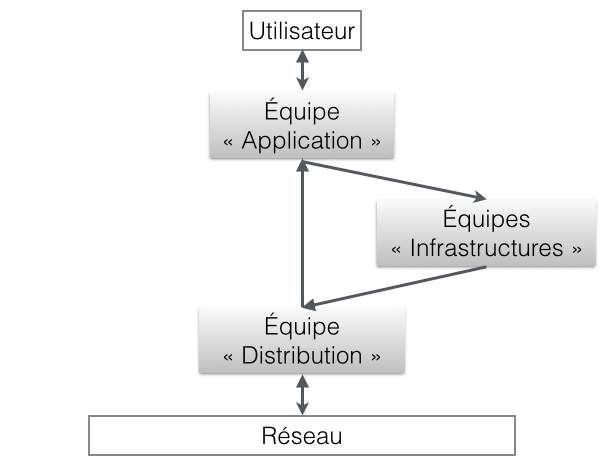
\includegraphics[scale=0.5]{IB.jpg}
\caption{Cheminement des messages entres les différentes équipes}
\end{center}
\end{figure}
		\subsubsection{IB2 Distribution}
Au sein d'IB, l'équipe IB2 Distribution a pour rôle d'assurer la distribution des messages depuis le réseau global jusqu'aux utilisateurs. 
\\

L'équipe est responsable d'une chaine de distribution constituée de trois composants majeurs. Le premier est un adaptateur qui convertit les messages du format du réseau vers le format interne à la chaine de distribution. Le second est un gestionnaire de versions qui assure la compatibilité des messages avec la version d'IB utilisée par le client.

Le dernier, IB Publisher, a pour rôle de publier les messages dans des emplacements de mémoire dédiés à leurs destinataires, appelé table. Ces tables, situées sur le réseau, sont enfin lues par l'application de l'utilisateur pour afficher les messages à l'écran.
\\

L'équipe a été créée il y a deux ans et demi pour concevoir IB Publisher, nouveauté structurelle d'IB2. Elle comptait quatre personnes il y a un an et en compte désormais neuf! Trois des membres sont des développeurs expérimentés (plus de vingt années d'expérience), quatre ont entre deux et six ans d'expérience et les deux derniers moins d'un an d'expérience.

Cette croissance s'explique par la volonté de repenser l'ensemble de la chaine de distribution. Dans cette optique, l'équipe a récupéré juste avant mon départ la responsabilité des deux autres composants de la chaine (l'adaptateur et le gestionnaire de version) sur lesquels elle travaillait déjà depuis plusieurs mois. Cela donnera à l'équipe plus de libertés pour effectuer les changements nécessaires à la restructuration de la distribution des messages.

Ce besoin est justifié par la forte croissance du nombre d'utilisateurs d'IB, qui impose d'améliorer les performances et la stabilité du système. En raison de l'ajout parfois précipité de fonctionnalités, le code a également besoin d'être repensé et simplifié.
	\subsection{Mission}
		\subsubsection{Objectifs}
L'équipe dispose actuellement de tests, dit unitaires, permettant de garantir le bon fonctionnement des sous-composants d'IB Publisher. En revanche, elle ne dispose pas de tests, dit d'intégration, permettant de prouver qu'une fois assemblés, ses sous-composants remplissent le cahier des charges de l'application.

Une des réalités de l'ingénierie logicielle est que nombre de développeurs sont réticents à écrire des tests. Cela s'explique sans doute par le fait que ces tests ne contribuent pas directement à l'expérience de l'utilisateur. Ils ne sont donc pas toujours considérés comme une partie intégrante du travail à réaliser et certains développeurs sous-entendent qu'écrire des tests ne fait que les ralentir dans leur travail.

Ces tests, unitaires ou d'intégration, sont pourtant essentiels dans un processus agile de développement. Ils permettent de développer itérativement les applications tout en assurant le bon fonctionnement des produits à toutes les étapes de la production. Ils garantissent en particulier le support des anciennes versions de l'application.
\\

Mon projet consistait donc en la création d'un environnement de tests d'intégration pour IB Publisher. Cet environnement devait tout d'abord garantir que les résultats des tests seraient le fait d'IB Publisher uniquement, et pas d'autres sous-composants. Pour cela, je devais isoler IB Publisher du reste de l'application, en créant des \textit{mocks} (i.e. des faux) reproduisant le comportement des autres sous-composants connectés à IB Publisher. Cette tache m'a occupé pendant les premières semaines de mon stage.

Je me suis ensuite consacré au développement du testeur en lui-même. Cette application devait être capable d'envoyer des messages puis de vérifier que les résultats obtenus dans les tables étaient conformes au cahier des charges d'IB Publisher.
		\subsubsection{Déroulement}
Lors de ma première semaine, mon tuteur était absent ce qui m'a laissé le temps d'apprendre les bases du C++. J'allais devoir utiliser ce langage de programmation dans la première partie de mon travail et il m'était inconnu à mon arrivée. Je me suis également familiarisé avec le fonctionnement d'IB et plus particulièrement d'IB Publisher et du gestionnaire de version. Ce gestionnaire sera appelé IB Version dans la suite de ce rapport.

La découverte de certaines parties du code a été déboussolante. Je n'étais en effet familier ni du langage ni des conventions utilisés. Je devais pourtant analyser le code d'IB Version afin d'en créer une copie simplifiée. L'équipe était très occupée cette semaine ci et ne disposait que de peu de temps pour m'aider à démarrer mon travail. J'ai alors du faire face à une sorte d'angoisse de la feuille blanche et je tardais à décider par où commencer.
\\

Au retour de mon tuteur, nous avons pu décider de l'architecture de mon projet et j'ai alors réellement démarré mon travail. Nous avons choisi de commencer par créer une reproduction simplifiée d'IB Version. La copie serait basée sur une technologie interne à Bloomberg, très utilisée par les développeurs. Cette technologie offre la possibilité à deux applications de communiquer très facilement et a donc permis d'assurer la connexion entre le testeur et le mock IB Version.

Cette technologie m'était tout à fait inconnue et étant interne à Bloomberg, je ne pouvais pas m'aider d'internet pour l'utiliser. Toute la semaine a donc été une lutte sur le plan technique pour parvenir à poser les fondations du mock IB Version.

La semaine suivante marquait le coup d'envoi du Summer Internship Program et était donc entièrement consacrée à des formations sur les outils et technologies utilisées à Bloomberg. Je m'absentais ensuite dix jours pour participer aux répétitions du 14 Juillet.
\\

À mon retour, j'ai réellement pu ressentir la plus value apportée par la formation et j'ai ainsi fait de rapides progrès sur la configuration initiale de mock IB Version. J'ai ensuite travaillé une semaine dans le but d'établir une connexion stable entre mock IB Version et IB Publisher.

Une fois ce travail terminé, je disposais des outils nécessaires pour démarrer la seconde phase de mon projet: le développement du testeur. Celui-ci enverrait des messages à mock IB Version, qui les transmettra à IB Publisher.
\\

La seconde partie de mon travail a été bien plus intéressante et enrichissante. Pour gagner en agilité, mon tuteur et moi-même avons en effet choisi de développer le testeur dans le langage Python. Ce langage est très facile d'accès et est largement utilisé ce qui fait d'Internet un outil puissant pour résoudre de nombreux problèmes. Ainsi, j'étais libéré des contraintes techniques que j'avais connues jusqu'alors et je pouvais réellement me concentrer sur le fond de mon travail.
\\
Mon tuteur et moi-même avons alors travaillé dans le but de créer une première version du testeur en portant une attention particulière à la clarté et à la qualité de l'architecture adoptée. Cet effort s'explique par le fait que mon travail devait être le plus simple possible à reprendre par le reste de l'équipe. Il s'agissait également d'un enjeu \og politique \fg{} pour mon tuteur qui souhaitait ainsi montrer au reste de l'équipe la nécessité de faire plus d'efforts sur ce point.

J'ai alors vraiment eu l'impression de pouvoir utiliser mes connaissances et mes qualités d'abstraction. Après deux semaines environ, je disposais d'une première version fonctionnelle du testeur.
\\

Mon ambition était ensuite de permettre aux développeurs de l'équipe d'écrire des tests sans avoir à écrire de code. Dans le temps qu'il me restait, j'ai donc développé une interface leur permettant de spécifier simultanément les messages faisant l'objet d'un test et les résultats attendus pour ces messages.
\begin{figure}
\begin{center}
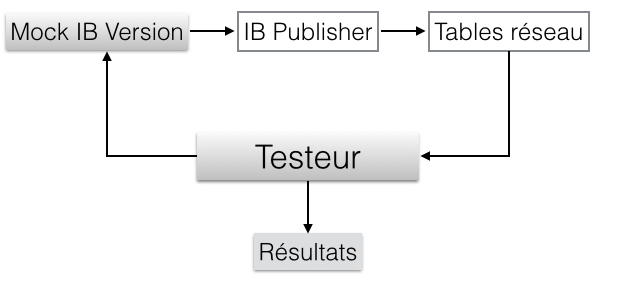
\includegraphics[scale=0.5]{testeur.jpg}
\caption{Architecture de l'environnement de test}
\end{center}
\end{figure}
		\subsubsection{Résultats et retours}
Un grand nombre de décisions relatives à l'orientation ou l'architecture du testeur ont été prises avec la participation de l'équipe tout entière. J'ai ainsi pu soumettre à plusieurs reprises mes réalisations et propositions à l'équipe et intégrer leurs avis et leurs besoins dans la suite de mon projet.

Lors de mes derniers entretiens avec eux, mon tuteur et mon chef d'équipe m'ont communiqué toute leur satisfaction quant au travail que j'avais réalisé. Ils ont également souligné mes efforts pour m'adapter rapidement aux outils et aux technologies utilisées dans l'environnement de travail.

Le testeur sera prochainement intégré à l'environnement de production d'IB. Ainsi, il sera possible de vérifier quotidiennement que les modifications apportées à IB Publisher n'impactent pas négativement le fonctionnement de l'application.
\\

La semaine de mon départ, un mini-forum était organisé pour permettre aux stagiaires de R\&D de présenter leurs travaux aux autres développeurs. Chacun d'entre nous pouvait ainsi présenter son projet de façon informelle.

J'ai alors réalisé que le problème que j'avais traité, à savoir tester une application publiant dans des tables sur le réseau, intéressait de nombreuses autres équipes. Plusieurs développeurs ont été très intéressés par le fonctionnement de mon application et vont rentrer en contact avec mon tuteur pour pouvoir l'adapter à leurs besoins.

Ces retours très positifs ont bien entendu été très gratifiants après plusieurs semaines de travail.
\newpage
\section{Enseignements}
Comme en témoigne ce rapport, ce stage qui constituait ma première expérience en entreprise a été particulièrement enrichissant sur le plan technique, personnel et professionnel. 
	\subsection{Enseignements techniques}
Sur plan technique, ce stage m'aura permis de découvrir de nouveaux outils et de nouvelles technologies mais surtout de découvrir les secteurs de l'ingénierie logicielle.
\\

J'ai donc entre autres appris deux nouveaux langages de programmation (C++ et Python) et je suis désormais familier avec plusieurs outils utilisés par tous les développeurs, comme le gestionnaire de versions Git. J'ai également découvert un certain nombre de technologies très utilisées actuellement, en particulier lors du hackathon auquel j'ai participé.

Dans un autre registre, j'ai consolidé ma culture en finance et j'ai travaillé mes méthodes de préparation aux entretiens d'embauche.
\\

Je me suis également familiarisé avec le secteur du développement informatique industriel et avec ses réalités.

Une des priorités permanente des développeurs est de concevoir un code durable. Contrairement aux projets menés en cours, chaque portion de code écrite doit ici être entretenue, parfois pendant plusieurs années. En plus d'être fiables et performants à l'instant présent, les produits conçus doivent être faciles à faire évoluer et à développer. Cette réalité est problématique pour certaines équipes très sollicitées, car elles ne disposent pas du temps nécessaire pour réaliser cet investissement.
\\

J'ai également acquis les bases de la conduite d'un projet informatique. J'ai ainsi appris à trouver le juste milieu entre la planification du développement et la découverte progressive des réalités du projet. J'ai également amélioré ma capacité à anticiper le temps nécessaire pour réaliser des changements et en particulier à anticiper les difficultés techniques.
	\subsection{Enseignements personnels} \label{ensperso}
Sur le plan personnel, cette expérience a été l'occasion de mesurer mes capacités d'adaptation. Par rapport aux autres stagiaires de R\&D, j'ai eu l'impression de m'être adapté plus rapidement aux valeurs et à l'esprit de la compagnie. Je ressentais particulièrement cette différence lors des événements interdépartements, cet esprit étant plus marqué en dehors de la R\&D.

J'ai cependant eu le sentiment d'avoir eu plus de difficultés qu'eux à m'adapter aux particularités du département. Je reconnais qu'avant mon arrivée, je considérais Bloomberg comme une compagnie financière et non technologique et que je n'étais donc pas préparé à rencontrer de telles spécificités.
\\

Comme pour beaucoup de stagiaires, mon projet était parallèle aux travaux actuels de l'équipe. Ceci permet aux stagiaires de pouvoir se familiariser plus sereinement avec les méthodes de travail que s'ils contribuaient directement au Terminal. À posteriori, je regrette de ne pas avoir pu contribuer au travail du reste de l'équipe.

J'ai évoqué ce regret avec mon tuteur. Celui-ci m'a répondu que plusieurs semaines de formation étaient nécessaires pour maitriser certains outils utilisés par l'équipe et que je n'aurais donc pas pu apporter une aide significative.
\\

Lors de la première phase de mon projet, mon travail nécessitait beaucoup de connaissances techniques que je ne possédais pas. Cela m'a donné le sentiment de ne pas pouvoir mettre à contribution mes qualifications et mes qualités et j'en ai été quelque peu frustré. Par la suite, j'ai toujours tenté d'organiser mon travail de façon à éviter cette situation.

Ainsi, j'ai eu le souci permanent d'anticiper la difficulté technique des tâches qui m'étaient confiées pour pouvoir demander en avance de l'aide au reste de l'équipe. Ceci m'a permis de progresser plus vite sur ces points et de pouvoir passer plus de temps sur des taches où je pouvais réellement ajouter de la valeur au projet.
\\

J'ai enfin pris conscience que les journées et les semaines passaient très vite ! Plus précisément, j'ai réalisé que sans effort particulier, les journées de travail peuvent se limiter à la réalisation des objectifs de court terme. Cela constitue selon moi un écueil à éviter à tout prix, et il faut en permanence chercher à inscrire son travail quotidien dans son projet personnel de long terme.

Dans le secteur du développement, la culture, la connaissance des technologies et l'amélioration continue de ses méthodes de travail sont essentielles. Il est ainsi crucial de consacrer du temps pour se former en continu. Après y avoir porté une attention particulière, j'ai eu le sentiment que cette \og conscience \fg{} était plus présente chez les développeurs expérimentés que chez les jeunes développeurs.
	\subsection{Orientation professionnelle}
Cette première immersion dans le secteur de l'ingénierie logicielle m'a enfin permis d'affiner mon projet professionnel.
\\

J'ai tout d'abord confirmé mon intérêt pour le développement informatique. Avant cette expérience, j'appréhendais quelque peu de passer des journées entières à coder mais j'ai finalement réalisé que le quotidien d'un développeur était bien plus varié. De plus, je passais en moyenne plus de temps à coder que le reste de l'équipe et je n'ai pas été \og lassé \fg{} par mon travail quotidien. Cette expérience me permet donc de confirmer mon choix de me spécialiser et de débuter ma carrière en ingénierie logicielle.
\\

L'observation des différentes personnes évoluant autour des développeurs m'a également permis de confirmer mon attrait pour la conduite de projet, la spécification des produits plus que leur conception, ou encore le design des infrastructures. Tous ces aspects sont utilisés comme \og matière première\fg{} par les développeurs, ce qui justifie de débuter ma carrière par une expérience de programmeur.

La conduite de projet m'intéresse particulièrement car elle implique de se consacrer à l'architecture des applications et permet de faire le lien entre les clients et les développeurs. Plus spécifiquement, je suis attiré par le travail de recherche consistant à spécifier les caractéristiques et le design d'une application à partir des retours et des demandes des clients. Ce travail nécessite d'anticiper les difficultés qui seront rencontrées par les programmeurs au moment du développement, mais également les besoins futurs du produit.
\newpage
\section{Conclusion}
\newpage
\section{Bibliographie}
\begin{description}
\item[Site de Bloomberg L.P.] \url{http://www.bloomberg.com/company}
\item[Site de Bloomberg Philanthropies] \url{http://www.bloomberg.org/}
\item[Article de presse comparant Bloomberg et Reuters] \url{http://www.investopedia.com/articles/investing/052815/financial-news-comparison-bloomberg-vs-reuters.asp}
\item[Wikipédia - Bloomberg L.P.] \url{https://en.wikipedia.org/wiki/Bloomberg_L.P.}
\item[Wikipédia - Michael Bloomberg] \url{https://en.wikipedia.org/wiki/Michael_Bloomberg}
\item[Wikipédia - Charles Zegar] \url{https://en.wikipedia.org/wiki/Charles_Zegar}
\end{description}
\end{document}
